\documentclass[PhysicsI/physics_notes.tex]{subfiles}
\begin{document}
\section{Aula 04 - 10/04/2023}
\subsection{Motivações}
\begin{itemize}
	\item Iniciar os estudos de movimentos em um plano todo (duas dimensões);
	\item Revisar vetores e sua manipulação.
\end{itemize}

\subsection{Vetores}
Começamos com um estudo das propriedades de veotres. Dados vetores $\vec{r_{1}}, \vec{r_{2}}$ e um número real $\lambda$, definimos:
\begin{itemize}
	\item[i)] A soma dos vetores:
	      \begin{center}
		      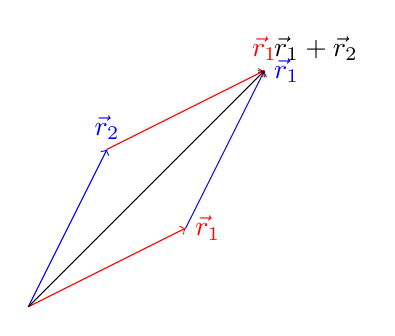
\begin{tikzpicture}
			      \coordinate (O) at (0,0); % origin
			      \draw [->,red] (O) -- (2,1) node [right] {$\vec{r}_1$}; % vector r_1
			      \draw [->,blue] (2,1) -- (3,3) node [right] {$\vec{r}_1$}; % vector r_1
			      \draw [->,blue] (O) -- (1,2) node [above] {$\vec{r}_2$}; % vector r_2
			      \draw [->,red] (1,2) -- (3,3) node [above] {$\vec{r}_1$}; % vector r_2
			      \draw [->,black] (O) -- (3,3) node [above right] {$\vec{r}_1+\vec{r}_2$}; % sum of vectors
		      \end{tikzpicture}
	      \end{center}
	\item[ii)] A multiplicação por escalar: $\lambda(r_{1}+r_{2})$ (Essencialmente, o resultado é aumentar ou diminuir o tamanho da seta.)
	      \begin{center}
		      \begin{tikzpicture}
			      \coordinate (O) at (0,0); % origin
			      \draw [->,red] (O) -- (2,1) node [right] {$\vec{v}$}; % vector v
			      \draw [->,blue] (O) -- (4,2) node [right] {$\lambda\vec{v}$}; % scaled vector
			      \draw [dashed] (2,1) -- (4,2); % dotted line to show scaling
		      \end{tikzpicture}
	      \end{center}
\end{itemize}
A título de curiosidade, a soma de vetores em três dimensões seria desta forma:
\begin{center}
	\tdplotsetmaincoords{70}{135} %set the viewing angle
	\begin{tikzpicture}[scale=2, tdplot_main_coords]
		\coordinate (O) at (0,0,0);
		\draw[thick,->] (O) -- (2,0,0) node[anchor=north east]{$x$};
		\draw[thick,->] (O) -- (0,2,0) node[anchor=north west]{$y$};
		\draw[thick,->] (O) -- (0,0,2) node[anchor=south]{$z$};

		\draw[->,red] (O) -- (1.5,0.5,1.5) node[midway, below right] {$\vec{u}$};
		\draw[->,blue] (1.5,0.5,1.5) -- (2,2,2) node[midway, above left] {$\vec{v}$};
		\draw[->,blue] (O) -- (0.5,1.5,0.5) node[midway, above] {$\vec{v}$};
		\draw[->,red] (0.5,1.5,0.5) -- (2,2,2) node[midway, below] {$\vec{u}$};
		\draw[->,black] (O) -- (2,2,2) node[midway, above right] {$\vec{u}+\vec{v}$};
	\end{tikzpicture}
\end{center}
Porém, não basta utilizar apenas representações gráficas para vetores. Desta forma, é comum definirmos um sistema de coordenadas
cartesiano para suas componentes. Assim, um vetor $\vec{u}$ pode ser decomposto em uma coordenada x e outra coordenada y:
$$
	\vec{u} = u_{x}\hat{i} + u_{y}\hat{j} (+u_{z}\hat{k})
$$
chamamos os valores $u_{x}, u_{y}, u_{z}$ de projeções, sendo a última um objeto presente apenas no caso de três coordenadas.
Com isso, definimos o módulo do vetor, ou seja, seu tamanho, pela fórmula
$$
	|\vec{u}| = \sqrt{u_{x}^{2}+u_{y}^{2}},
$$
e, de brinde, ganhamos fórmulas para as projeções em cada coordenada:
\begin{align*}
	 & u_{x} = |u|\cos{\theta} \Rightarrow \cos{\theta} = \frac{u_{x}}{|\vec{u}|} \\
	 & u_{y} = |u|\sin{\theta} \Rightarrow \sin{\theta} = \frac{u_{y}}{|\vec{u}|} \\
	 & \tan{\theta} = \frac{u_{y}}{u_{x}}.
\end{align*}
é importante, tamém, darmos uma forma de obter um betor de módulo 1, i.e., um vetor unitário, visto que ele pode nos fornecer a informação do
valor do ângulo $\theta$, a direção, etc. Ele é obtido reduzindo um vetor u pelo seu módulo,
$$
	\hat{u} = \frac{\vec{u}}{|\vec{u}|}.
$$
Uma utilidade imediata da definição em coordenadas é que agora temos um modo de tratar a soma de vetores algebricamente
\begin{align*}
	 & \text{Soma: } \vec{u}+\vec{v} = (u_{x}\hat{i} + u_{y}\hat{j}) + (v_{x}\hat{i} + v_{y}\hat{j}) = (u_{x}+v_{x})\hat{i} + (u_{y}+v_{y})\hat{j} \\
	 & \text{Multiplicação por Escalar: } \lambda \vec{u} = \lambda(u_{x}\hat{i} + u_{y}\hat{j}) = \lambda u_{x}\hat{i} + \lambda u_{y}\hat{j}     \\
	 & \theta = ctg{\biggl(\frac{\lambda u_{y}}{\lambda u_{x}}\biggr) = ctg{\biggl(\frac{u_{y}}{u_{x}}\biggr)}}.
\end{align*}
Agora podemos ir à aplicação física dessa discussão, o deslocamento de uma partícula no plano. Nesta configuração, normalmente
terá-se uma partícula com posição $\vec{x}(t) = x(t)\hat{i} + y(t)\hat{j}\quad (+z(t)\hat{k}).$ Para realizar o estudo desses casos,
vamos decompor o movimento dela em cada eixo, ou seja, quebramos o movimento no plano em dois movimentos independentes, um em cada eixo
x ou y. Nestas condições, o deslocamento de uma partícula de uma posição 1 até uma posição 2 será
$$
	\vec{x_{2}} - \vec{x_{1}} = (x_{2}\hat{i} + y_{2}\hat{j}) - (x_{1}\hat{i}+y_{1}\hat{j}) = (x_{2}-x_{1})\hat{i} + (y_{2}-y_{1})\hat{j}.
$$
Com isso, podemos escrever que o deslocamento $\Delta \vec{r}$ é
$$
	\Delta \vec{r} = \Delta x\hat{i} + \Delta y\hat{j}.
$$
Ainda mais, se conhecemos o valor do ângulo entre as posições 1 e 2 e o módulo dos vetores representando-as,
$$
	|\Delta r|^{2} = x_{1}^{2} + x_{2}^{2} - 2x_{1}x_{2}\cos{\theta}.
$$
Tendo o básico do deslocamento, podemos repetir o raciocínio prévio para trabalhar com aceleração e velocidade. De fato,
$$
	\vec{v_{m}} = \frac{\Delta \vec{r}}{\Delta t}, \quad \vec{a_{m}} = \frac{\Delta \vec{v_{m}}}{\Delta t}
$$
e os valores instantâneos serão dados por
\begin{align*}
	 & \vec{v}(t) = \frac{d \vec{r}(t)}{dt} = \frac{d x(t)}{dt}\hat{i} + \frac{d y(t)}{dt}\hat{j} = v_{x}\hat{i} + v_{y}\hat{j}.         \\
	 & \vec{a}(t) = \frac{d \vec{v}(t)}{dt} = \frac{d v_{x}(t)}{dt}\hat{i} + \frac{d v_{y}(t)}{dt}\hat{j} = a_{x}\hat{i} + a_{y}\hat{j}.
\end{align*}
Além disso, o módulo e orientação desses valores serão dados por
\begin{align*}
	 & |\vec{v}| = \sqrt{v_{x}^{2}+v_{y}^{2}},\quad \theta_{v} = ctg\biggl(\frac{v_{y}}{v_{x}}\biggr)  \\
	 & |\vec{a}| = \sqrt{a_{x}^{2}+a_{y}^{2}},\quad \theta_{a} = ctg\biggl(\frac{a_{y}}{a_{x}}\biggr).
\end{align*}
Note que a aceleração não aponta na direção da velocidade em si, mas sim na direção da \textbf{variação} da velocidade.

\subsection{Movimento Uniforme Bidimensional}
Considere uma partícula com posição $\vec{r}(t)$ e uma orientação, tal que forma um ângulo $\theta$ com o plano. Como
estaremos considerando o movimento do tipo uniforme, a aceleração é nula e a velocidade $\vec{v}(t) = v_{0}$ é constante,
tendo módulo $v_{0}$ e orientação $\theta$. Em outras palavras, as componentes desse vetor serão, também, constantes, isto é,
$$
	\text{constantes}\left\{\begin{array}{ll}
		v_{x}(t) = v_{x_{0}} \\
		v_{y}(t) = v_{y_{0}}.
	\end{array}\right.
$$
Desta forma, a decomposição da velocidade em coordenadas é tal que
\begin{align*}
	 & \text{Eixo x: }v_{x}(t) = v_{x_{0}} \Rightarrow x(t) = x_{0} + v_{x_{0}}(t-t_{0}),\quad x_{0} = x(t_{0})  \\
	 & \text{Eixo y: }v_{y}(t) = v_{y_{0}} \Rightarrow y(t) = y_{0} + v_{y_{0}}(t-t_{0}),\quad y_{0} = y(t_{0}).
\end{align*}
Logo, a posição da partícula no plano será dada por
$$
	\vec{r}(t) = x(t)\hat{i} + y(t)\hat{j} = (x_{0} + v_{x_{0}}(t-t_{0})\hat{i}) + (y_{0} + v_{y_{0}}\hat{j}).
$$
Note que, quando falamos de trajetória de uma partícula ou objeto, buscamos uma relação entre as componentes x(t) e y(t) que
independe do tempo, isto é, a relação temporal é dada de forma implicita. Uma forma de fazer isso é a através da tangente, pois
$$
	\frac{y(t) - t_{0}}{x(t) - x_{0}} = \frac{v_{y_{0}}(t-t_{0})}{v_{x_{0}}(t-t_{0})} = \frac{v_{y_{0}}}{v_{x_{0}}} = \tan{\theta_{0}}.
$$
Com isso,
$$
	y(t) - y_{0} = \tan{\theta_{0}}(x(t)-x_{0}) \Rightarrow y = \tan{(\theta_{0})}x - \tan{(\theta_{0})}x_{0} + y_{0},
$$
ou seja, y tem a forma de um eluação da reta com inclinação constante e igual a $\tan{\theta_{0}}.$
\end{document}
